\documentclass[tikz,border=3.14mm]{standalone}
\usepackage{pgfplots}

\begin{document}
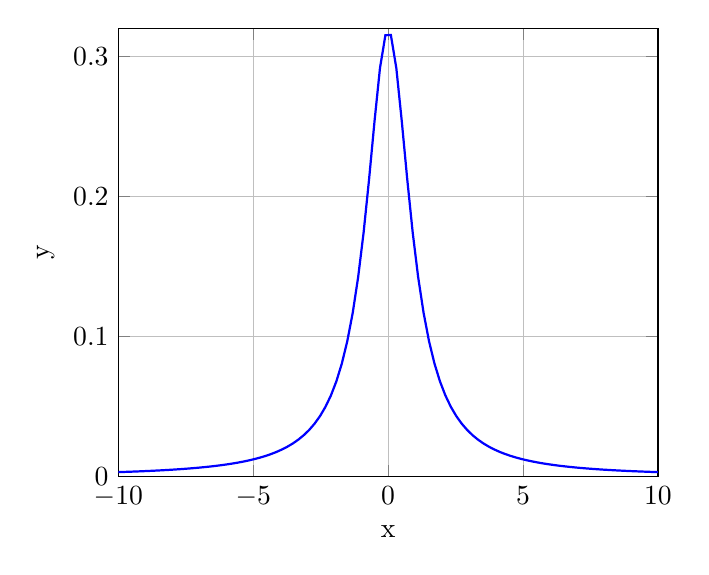
\begin{tikzpicture}
\begin{axis}[
    xlabel={x},
    ylabel={y},
    xmin=-10, xmax=10,
    ymin=0, ymax=.32,
    xtick={-10,-5,0,5,10},
    ytick={0,0.1,0.2,0.3},
    grid=both,
    grid style={line width=.1pt, draw=gray!10},
    major grid style={line width=.2pt,draw=gray!50},
    % axis lines=middle,
    samples=100,
]

% Original wiggly non-negative function (like sin(x) convolved with a wide normal distribution)
\addplot[blue, thick, domain=-10:10] {1/(pi*1*(1+((x)/1)^2))};

\end{axis}
\end{tikzpicture}
\end{document}